\documentclass[11pt,a4paper]{article}

\usepackage[margin=1in]{geometry}
\usepackage{amsmath, amssymb, mathtools}
\usepackage{fontspec}
\IfFontExistsTF{Times New Roman}
  {\setmainfont{Times New Roman}}
  {\setmainfont{Liberation Serif}}
\IfFontExistsTF{Arial}
  {\setsansfont{Arial}}
  {\setsansfont{Liberation Sans}}
\usepackage{newunicodechar}
\newunicodechar{≈}{\ensuremath{\approx}}
\newunicodechar{≤}{\ensuremath{\leq}}
\newunicodechar{≥}{\ensuremath{\geq}}
\newunicodechar{×}{\ensuremath{\times}}
\newunicodechar{−}{\ensuremath{-}}

\usepackage{xcolor}
\definecolor{headingcolor}{HTML}{1F4E79}
\definecolor{lightgray}{HTML}{666666}

\usepackage{setspace}
\onehalfspacing
\setlength{\parindent}{0pt}
\setlength{\parskip}{0.6em}

\usepackage{titlesec}
\titleformat{\section}
{\color{headingcolor}\sffamily\Large\bfseries}
{\thesection}{1em}{}
\titleformat{\subsection}
{\sffamily\large\bfseries}
{\thesubsection}{1em}{}

\usepackage{listings}
\lstset{
    basicstyle=\ttfamily\footnotesize,
    breaklines=true,
    columns=fullflexible,
    frame=single,
    framerule=0.4pt,
    showstringspaces=false,
    xleftmargin=0.4em,
    xrightmargin=0.4em,
    aboveskip=0.5em,
    belowskip=0.5em,
}

\usepackage{booktabs}
\usepackage{graphicx}
\usepackage{caption}
\captionsetup{font=small, labelfont=bf}

\newcommand{\courseheader}{
    \begin{center}
        {\sffamily\Large\bfseries CESE5040}\\[0.3em]
        {\sffamily High-Performance and AI Architectures}\\
        {\color{lightgray}2026 Q4}
    \end{center}
}

\newcommand{\Q}[1]{\subsection*{Question #1}}
\newcommand{\Qpart}[1]{\textbf{#1.}}

\begin{document}

\courseheader
\vspace{1em}

{\color{headingcolor}\sffamily\large\bfseries Student Information}

\textbf{Name:} Daniel Tyukov\\
\textbf{Student Number:} 5714699\\
\textbf{Lab:} Lab Assignment 3

{\color{headingcolor}\sffamily\large\bfseries Notes}

\begin{itemize}
    \item Hardware: same AWS course VM as previous labs
    (Intel Xeon Platinum 8375C, 4 physical cores / 8 vCPUs, 15 GiB RAM)
    plus an attached \textbf{NVIDIA Tesla T4} (15 GiB, sm\_75, CUDA 13.0
    driver 580.126.09).
    \item Software: Python 3.12, NumPy 2.x, CuPy 14.0.1, Numba 0.65.0,
    JAX 0.10.0, nvprof from the CUDA toolkit, all double precision.
    \item Each timing is the minimum of 3 runs after one warm-up. GPU
    timings include a \texttt{cuda.synchronize()} both before timer start
    and at the end so we measure full kernel completion, not just submit.
    \item Submitted code: \texttt{L3\_Q1.py}, \texttt{L3\_Q2.py},
    \texttt{L3\_Q4.py}, \texttt{L3\_Q5.py}. \texttt{tvb\_vec\_full.py} is
    the fully refactored NumPy version that L3\_Q1 is built on.
    \item Sanity check: each implementation reproduces \texttt{tvb\_vec.py}
    on TVB76/5~ms to within $\approx 3 \times 10^{-15}$ (FP reordering noise).
\end{itemize}

\vspace{0.5em}

\section*{\color{headingcolor}Lab Exercise 3}

\Q{3.1 — TVB on GPU using CuPy}

\Qpart{1, 2, 3} Times for the unmodified \texttt{tvb\_vec.py}, the fully
vectorised NumPy version (\texttt{tvb\_vec\_full.py}), and the CuPy port
(\texttt{L3\_Q1.py}) on all three datasets at \texttt{tf}=150~ms:

\begin{table}[h]
\centering
\small
\begin{tabular}{lrrr}
\toprule
Implementation & TVB76 (s) & TVB192 (s) & TVB998 (s) \\
\midrule
\texttt{tvb\_vec.py} (baseline)              & \textbf{9.30}    & \textbf{23.81}   & \textbf{172.43} \\
\texttt{tvb\_vec\_full.py} (no per-N loop)   & \textbf{0.41}    & \textbf{1.76}    & \textbf{57.50}  \\
\texttt{L3\_Q1.py} (CuPy on Tesla T4)        & \textbf{1.90}    & \textbf{1.92}    & \textbf{3.04}   \\
\bottomrule
\end{tabular}
\caption{Wall time, min of 3 reps, 150~ms simulation, dt=0.05.}
\end{table}

\Qpart{4} \textit{Discussion.} The first refactor (vec\_baseline →
vec\_full) is the biggest single jump on the small datasets. Removing
the per-centre Python loop turns $N \cdot T$ NumPy calls into $T$
NumPy calls, and the per-call dispatch overhead was where most of the
time was sitting at $N=76$. At TVB998 the speedup shrinks to about
$3\times$ because the actual $\mathcal{O}(N^2)$ NumPy work has taken
over from the dispatch cost.

The CuPy numbers were a surprise at first. TVB76 and TVB192 are not
faster than plain NumPy, and TVB76 is actually slower (1.90~s vs
0.41~s). The simulation is 3000 timesteps, each one launches around
22 small CuPy kernels, and on a T4 each launch costs roughly 6--10~µs.
That is already $\approx 0.5$~s of pure launch overhead before any
real arithmetic, and at TVB76 the GPU finishes the actual work in
well under that.

CuPy only wins on TVB998, where the coupling sum is a 998×998 matmul
instead of 76×76 and each step has enough work to saturate the GPU.
There it lands at 3.04~s, about $19\times$ faster than vec\_full at
57.5~s. Figure~\ref{fig:scaling} shows the same picture across all
six implementations.

\begin{figure}[h]
\centering
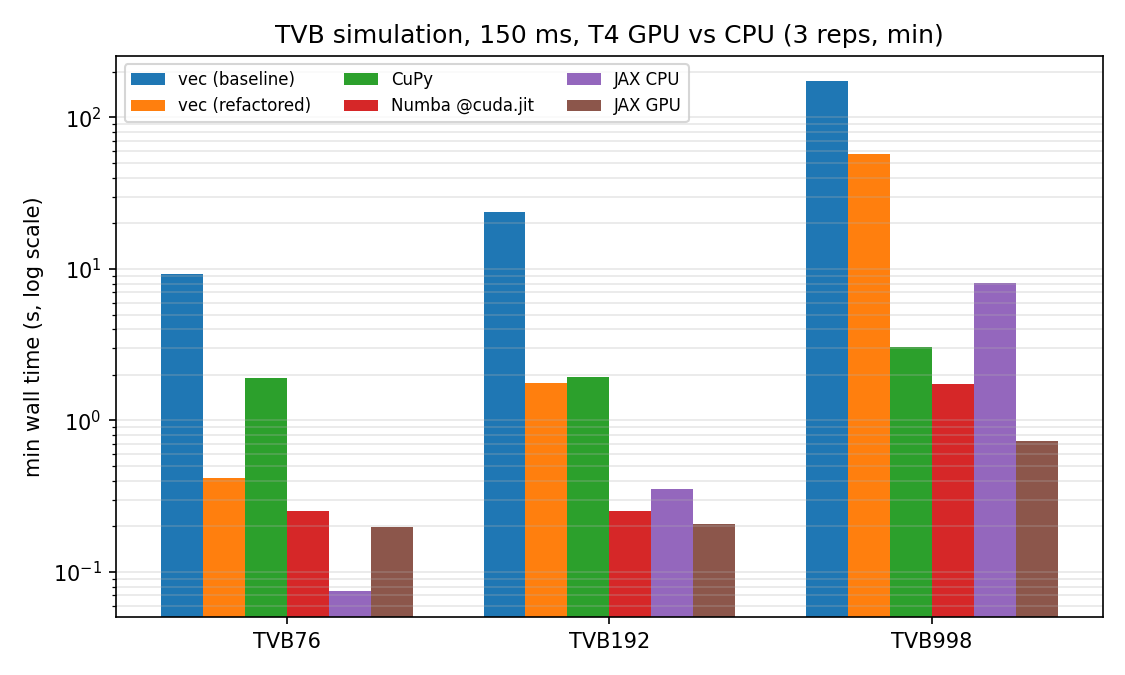
\includegraphics[width=0.85\linewidth]{../figures/scaling_dataset.png}
\caption{Wall time across all six implementations, log scale. CuPy
loses to vec\_full at TVB76, breaks even at TVB192, and wins by
~19$\times$ at TVB998.}
\label{fig:scaling}
\end{figure}

\textit{What if we hadn't refactored in step~2?} The CuPy version
would be much worse, not better. Each of the $N$ inner iterations
would launch its own bundle of CuPy kernels, so for TVB998 that's
$998 \cdot 3000 \approx 3$M kernel launches per run. At 6~µs each
that's 18~s of pure launch latency before the GPU does any real work,
and the per-launch work shrinks to one row of the coupling sum, which
also tanks GPU occupancy. Refactoring before porting wasn't optional.

\Qpart{5} \textit{nvprof profile.} Nsys 2022.4 on the VM can record
\texttt{.qdstrm} files but its importer is missing, so I used
\texttt{nvprof} for the textual breakdown instead. Run on TVB192,
single rep, no warmup:

\begin{figure}[h]
\centering
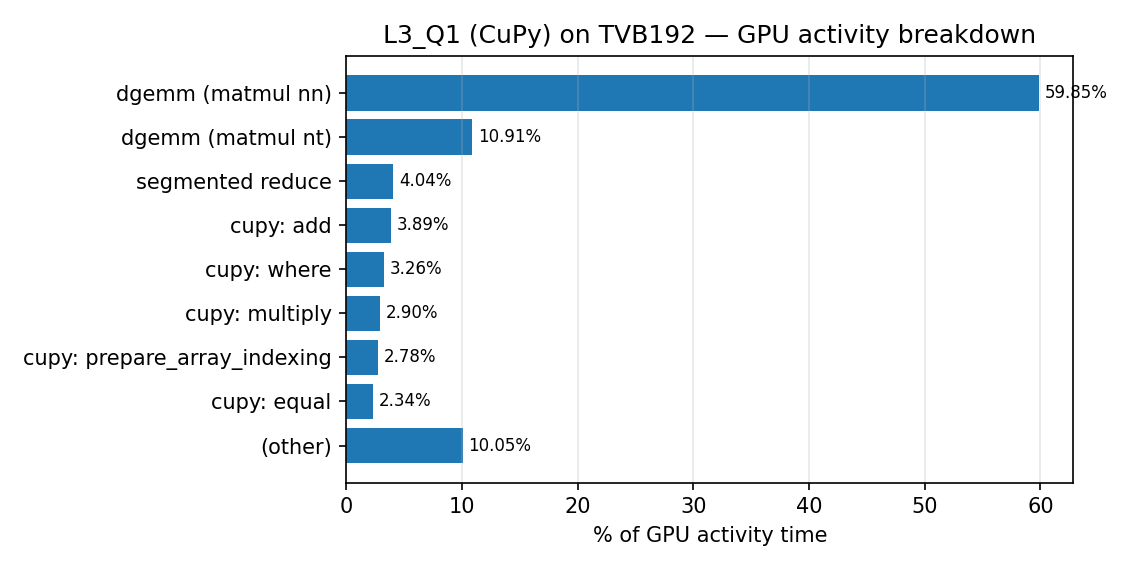
\includegraphics[width=0.85\linewidth]{../figures/q15_breakdown.png}
\caption{\texttt{nvprof} GPU activity breakdown for L3\_Q1 on TVB192,
150~ms. Two cuBLAS dgemm kernels (the MLP matmuls) take 70.8\% of all
GPU time on their own.}
\end{figure}

The two dgemm calls per step (the [N,2]·[2,64] and [N,64]·[64,2]
matmuls inside the MLP) dominate at 70.8\% of GPU activity. The
segmented reduce is the row-sum in the coupling step, the rest is
small element-wise kernels. As for data movement: nvprof reports a
single \texttt{[CUDA memcpy HtoD]} category at \textbf{101.69~µs}
total over 6 calls, plus a few small \texttt{[CUDA memset]}s
(8.4~ms). There is no \texttt{[CUDA memcpy DtoH]} during the timed
loop because we keep \texttt{Xs} on the GPU and never copy it back
inside \texttt{simulate\_gpu}. Total GPU activity time was about
966~ms, so data movement is roughly \textbf{0.01\%} of GPU time and a
similarly tiny fraction of the 3.3~s wall. The wall-time gap above the
GPU activity time (3.3~s vs 0.97~s) is launch latency from
\texttt{cuLaunchKernel}, not transfers.

\Q{3.2 — High-throughput TVB on GPU (\texttt{L3\_Q2.py})}

\textbf{Implementation.} I added a leading $K$ axis to every state and
output array. \texttt{Xs} is now \texttt{[K, N, M, T]}, the MLP matmul
becomes a batched \texttt{[K, N, M] @ [M, L]} (NumPy/CuPy do this
automatically), and the coupling indices are computed once per step
and broadcast across $K$. $W$ and $D$ are uploaded to the GPU exactly
once and reused for every simulation.

\begin{table}[h]
\centering
\small
\begin{tabular}{lrrrr}
\toprule
$K$ & Wall (s) & Throughput (iters/s) & Back-to-back L3\_Q1 (s) & Throughput (iters/s) \\
\midrule
100 & \textbf{7.42}  & \textbf{40,412} & 192.0  & 1,562 \\
250 & \textbf{18.15} & \textbf{41,314} & 480.1  & 1,562 \\
500 & \textbf{36.20} & \textbf{41,439} & 960.2  & 1,562 \\
\bottomrule
\end{tabular}
\caption{TVB192, 150~ms (3000 timesteps per simulation). Back-to-back
L3\_Q1 numbers are extrapolated as $K \cdot 1.92$~s using the TVB192
single-sim time from Q3.1.}
\end{table}

\begin{figure}[h]
\centering
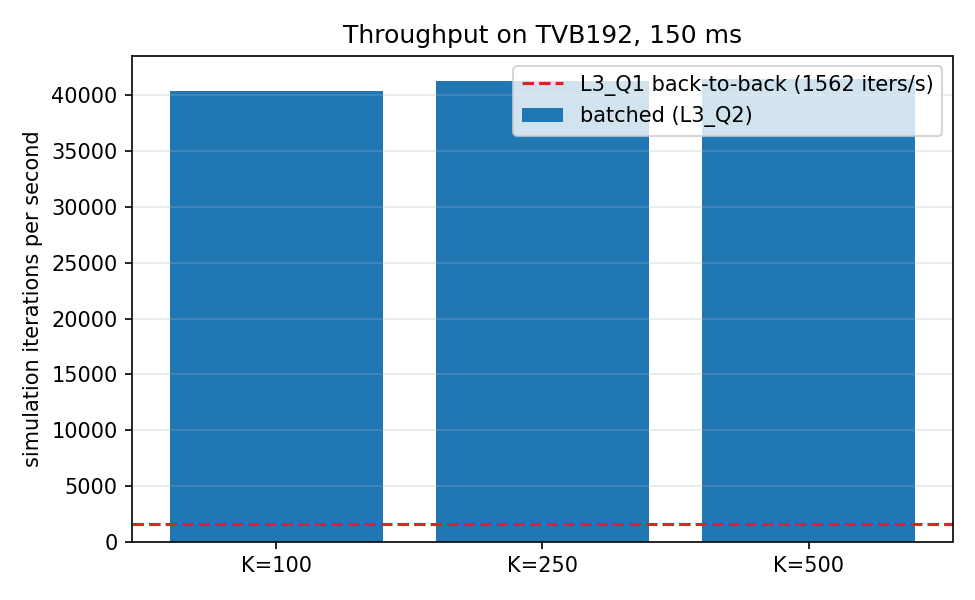
\includegraphics[width=0.65\linewidth]{../figures/throughput_q2.png}
\caption{Iterations per second on the same GPU, batched vs running
L3\_Q1 sequentially $K$ times.}
\end{figure}

\textbf{Which is better and why?} Batched, by about $26\times$ at every
$K$. The reason is the launch-overhead story from Q3.1, but flipped on
its head: when you run L3\_Q1 sequentially you pay $T \cdot K \cdot
(\text{launches per step})$ kernel launches in total, and at TVB192
each individual kernel only does about 192 nodes of work, which is way
below saturation for a T4. Batching keeps the same number of launches
($T \cdot \text{launches per step}$, no $K$) and just makes each
kernel $K$ times bigger, so the SMs actually fill up. The per-step
matmul becomes $[K\cdot N, 2] @ [2, 64]$ which is a real piece of
work. Throughput rises from 1.56k iters/s to 41k iters/s
($\approx 26\times$) and stays roughly flat from $K=100$ on, which
suggests the T4 is now saturated and the only thing growing with $K$
is the wall time.

\Q{3.3 — nvprof of L3\_Q2}

\begin{figure}[h]
\centering
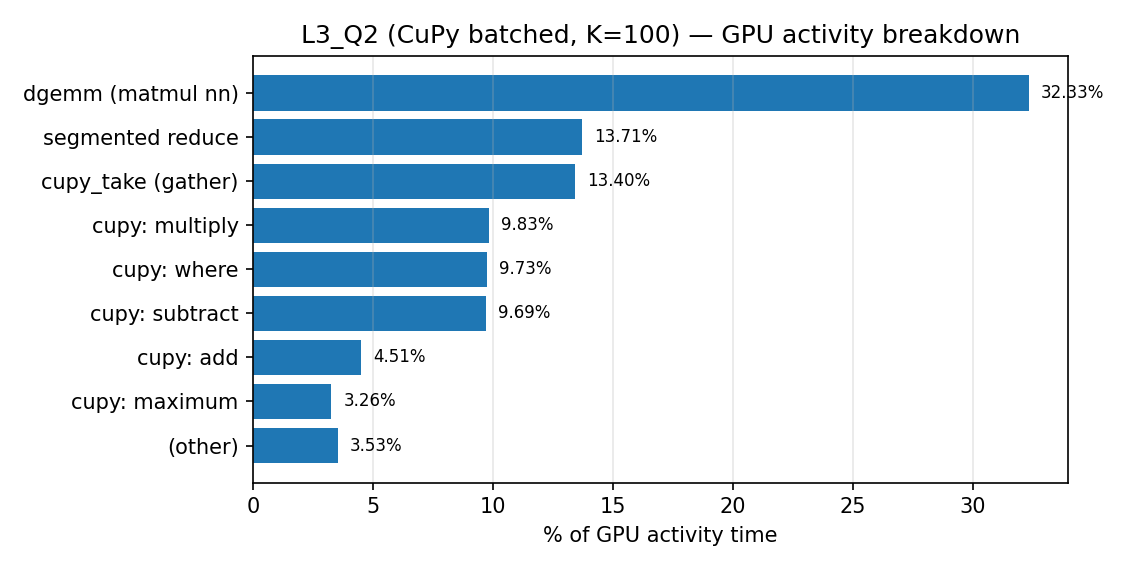
\includegraphics[width=0.85\linewidth]{../figures/q33_breakdown.png}
\caption{nvprof breakdown of L3\_Q2 on TVB192, $K=100$, 150~ms.}
\end{figure}

The same kernels appear, but the proportions shift: dgemm goes from
71\% (single sim) to 32\%, and the gather (\texttt{cupy\_take}) and
its surrounding element-wise kernels (multiply, where, subtract) take
a much bigger slice. That makes sense, since every per-step
element-wise op now does $K\cdot N$ elements of work instead of $N$
and so grows linearly with $K$, while the dgemm cost grows
sub-linearly because the batched dgemm is more efficient.

Data movement: again a single \texttt{[CUDA memcpy HtoD]} block at
\textbf{101.69~µs} (the W/D upload at the start), no DtoH inside the
timed region, and \texttt{[CUDA memset]} contributes 8.2~ms. Total GPU
activity was about 7.5~s, so data movement is around \textbf{0.001\%}
of GPU time. Once state lives on the GPU, transfers are not the
bottleneck. Kernel launches and per-step element-wise work are.

\Q{3.4 — TVB on GPU with Numba \texttt{@cuda.jit} (\texttt{L3\_Q4.py})}

\textbf{Implementation.} I wrote one \texttt{@cuda.jit} kernel that
runs a full timestep. Each thread handles one brain region: it walks
all $N$ source nodes to compute the coupling sum into a register, runs
the [2 → 64 → 2] MLP fully unrolled (also in registers), adds the
coupling to the second output, and writes the new $[x, y]$ back into
\texttt{Xs[n, :, t]}. The timestep loop is in Python and just launches
the kernel $T-1$ times. Threads only ever write disjoint slots in
\texttt{Xs} so I don't need atomics, shared memory or any extra
synchronisation.

\begin{table}[h]
\centering
\small
\begin{tabular}{lrrr}
\toprule
Implementation & TVB76 (s) & TVB192 (s) & TVB998 (s) \\
\midrule
L3\_Q1 (CuPy)            & \textbf{1.90} & \textbf{1.92} & \textbf{3.04} \\
L3\_Q4 (Numba cuda.jit)  & \textbf{0.25} & \textbf{0.25} & \textbf{1.74} \\
\midrule
speedup vs CuPy          & 7.5$\times$  & 7.7$\times$  & 1.7$\times$ \\
\bottomrule
\end{tabular}
\caption{Single-simulation runtime, 150~ms.}
\end{table}

Numba is faster than CuPy across the board. The main reason is the
launch count: CuPy issues about 22 kernels per timestep (one per
NumPy-style op), Numba issues exactly one. With $T=3000$ timesteps and
a per-launch cost of $\approx 6$~µs that alone is around 0.4~s saved.
The gap shrinks at TVB998 because there the actual $N^2$ coupling work
inside each kernel becomes the bottleneck rather than the launch
overhead, and at that point cuBLAS \texttt{dgemm} (what CuPy uses) is
genuinely faster than my hand-written nested loop. Even so Numba is
still about $1.7\times$ faster overall because the same launch-count
saving applies.

\textbf{Multi-simulation version.} The kernel as written assumes
\texttt{Xs} is shape \texttt{[N, M, T]} and uses 1D \texttt{cuda.grid(1)}
indexing. To run $K$ sims at once I would:

\begin{itemize}
    \item Allocate \texttt{Xs} as \texttt{[K, N, M, T]} (and pre-fill the
    \texttt{[:, :, :, 0] = -1.0} initial condition for all $K$).
    \item Switch to a 2D grid:
    \texttt{kernel[((N+TPB-1)//TPB, K), (TPB, 1)](\dots)} so that
    \texttt{n = cuda.blockIdx.x * cuda.blockDim.x + cuda.threadIdx.x}
    indexes the brain region and \texttt{k = cuda.blockIdx.y} indexes
    the simulation. Inside the kernel every \texttt{Xs[\dots]} access
    gains a leading \texttt{[k]} index. $W$ and $D$ stay shared across
    all $K$.
    \item Keep the timestep loop in Python so all $K\cdot N$ threads
    finish step $t$ before $t+1$ starts (the kernel-launch boundary
    is the per-timestep barrier).
\end{itemize}

The $W, D$ matrices are read-only and identical across simulations, so
nothing needs to change for them. There is also no inter-simulation
coupling so no atomics either.

\Q{3.5 — TVB with JAX (\texttt{L3\_Q5.py})}

\textbf{Implementation.} The simulation function is the same shape as
\texttt{L3\_Q1.py}'s \texttt{simulate\_gpu}, but rewritten in JAX
functional style. The Python timestep loop becomes a
\texttt{jax.lax.scan} so that the whole simulation compiles into a
single XLA program; \texttt{Xs.at[:, :, t].set(new\_X)} replaces the
in-place write, conditionals on validity become \texttt{jnp.where}, and
the function is wrapped in \texttt{@jax.jit}. The backend is selected
via the \texttt{JAX\_PLATFORMS} env var (\texttt{cpu} or \texttt{cuda})
before \texttt{jax} is imported. \texttt{x64} is enabled per the
assignment hint.

\begin{table}[h]
\centering
\small
\begin{tabular}{lrrr}
\toprule
Implementation & TVB76 (s) & TVB192 (s) & TVB998 (s) \\
\midrule
NumPy (vec\_full)        & 0.41 & 1.76  & 57.50 \\
CuPy (L3\_Q1)            & 1.90 & 1.92  & 3.04 \\
Numba @cuda.jit (L3\_Q4) & 0.25 & 0.25  & 1.74 \\
JAX (CPU)                & \textbf{0.07} & 0.35  & 8.03 \\
JAX (GPU)                & 0.20 & \textbf{0.21}  & \textbf{0.73} \\
\bottomrule
\end{tabular}
\caption{Single-simulation wall time, 150~ms, min of 3 reps after one
warmup. Warmup matters for JAX because the first call triggers the XLA
compile.}
\end{table}

JAX CPU is the fastest CPU implementation at every dataset: 74~ms on
TVB76 vs vec\_full's 414~ms ($5.6\times$), 0.35~s vs 1.76~s on
TVB192 ($5\times$), 8.03~s vs 57.5~s on TVB998 ($7.2\times$). XLA
fuses the entire scan body into one compiled function, so the
per-step Python dispatch into many small NumPy ops disappears.

JAX GPU is the fastest implementation overall on TVB998 at 0.73~s,
beating Numba's \texttt{@cuda.jit} (1.74~s) and CuPy (3.04~s). On
TVB76 it loses slightly to JAX-CPU, because launch and small-kernel
overhead dominate a 76-node problem, but it stays in the same
ballpark as Numba.

What's nice is that the same source file runs both backends with no
code changes, just a different value of \texttt{JAX\_PLATFORMS}.
That matches what the assignment description advertises about JAX
as a portable layer.

The reason JAX-GPU wins on TVB998 is fusion. XLA can take the whole
scan body and emit a small set of fused kernels per step instead of
CuPy's 22 separate ones, and unlike Numba it can use cuBLAS for the
heavy matmul rather than an unrolled inner loop. On TVB998 those two
effects compound. On TVB76/192 the GPU cost is dominated by launches
and the small kernels, so the three GPU backends end up close to
each other.

\vspace{1em}

% LLM Disclosure
{\color{headingcolor}\sffamily\large\bfseries LLM Usage Disclosure}

\vspace{0.3em}

I used Claude Code on this lab for:
\begin{itemize}
    \item Cross-checking the JAX scan / functional-update idioms
    against the JAX docs while porting from the NumPy version.
    \item Editing the report (cutting filler, tightening phrasing).
\end{itemize}

\end{document}
